\documentclass[a4paper,fleqn,usenatbib]{mnras}
\pdfoutput=1
% MNRAS is set in Times font. If you don't have this installed (most LaTeX
% installations will be fine) or prefer the old Computer Modern fonts, comment
% out the following line
%\usepackage{newtxtext,newtxmath}
% Depending on your LaTeX fonts installation, you might get better results with one of these:
%\usepackage{mathptmx}
%\usepackage{txfonts}

% Use vector fonts, so it zooms properly in on-screen viewing software
% Don't change these lines unless you know what you are doing
\usepackage[T1]{fontenc}
\usepackage{ae,aecompl}
\usepackage{epstopdf}
\usepackage{aas_macros}
\usepackage{braket}
\usepackage{verbatim}
\usepackage{wrapfig}
\usepackage{booktabs}
\usepackage{amsfonts}
\usepackage{amsmath}
\usepackage{appendix}
\usepackage{graphicx}
\usepackage[usenames,dvipsnames]{color}
\usepackage[normalem]{ulem}
\usepackage{array}
\bibliographystyle{mnras}


\newcommand{\myemail}{samuelreay@gmail.com}
\newcommand{\tick}{\checkmark}
\newcommand{\gtick}{\color{ForestGreen} \tick }
\newcommand{\cross}{$\times$ }
\newcommand{\rcross}{\color{red} \cross }
\newcommand{\runz}{\textsc{Runz}}
\newcommand{\brac}[1]{\left( #1 \right)}
\newcommand*\mean[1]{\bar{#1}}
\newcommand\abs[1]{\left|#1\right|}
\newcommand {\etal} {\emph{~et~al.} }
\newcommand{\green}{\color{green}}
\newcommand{\blue}{\color{blue}}
\newcommand{\red}{\color{red}}
\newcommand{\orange}{\color{BurntOrange}}
\newcommand{\purple}{\color{Fuchsia}}
\newcommand{\hMpc}{h^{-1} {\rm Mpc}} % to be used in math mode
\newcommand{\camb}{\textsc{camb}}
\newcommand{\cosmomc}{\textsc{cosmomc}}

\newcommand{\kmsmpc}{km\,s$^{-1}$\,Mpc$^{-1}$}

\newcommand{\halofit}{\textsc{halofit}}
\newcommand{\specialcell}[2][c]{\begin{tabular}[#1]{@{}c@{}}#2\end{tabular}}



%\shortauthors{}
\title[MC Corrections for Bayesian Methods]{Monte Carlo Corrections for Bayesian Methods}

\author[S. R. Hinton et al.]{Samuel R. Hinton,$^{1,2}$\thanks{E-mail: \href{samuelreay@gmail.com}}
\\
% List of institutions
$^{1}$School of Mathematics and Physics, The University of Queensland, Brisbane, QLD 4072, Australia\\
$^{2}$ARC Centre of Excellence for All-sky Astrophysics (CAASTRO)
}
% These dates will be filled out by the publisher
\date{Accepted XXX. Received YYY; in original form ZZZ}

% Enter the current year, for the copyright statements etc.
\pubyear{2017}

\begin{document}


\label{firstpage}
\pagerange{\pageref{firstpage}--\pageref{lastpage}}
\maketitle



\begin{abstract}
Lifetimes are strictly positive. Fainter objects are harder to see with a telescope than brighter ones. We cut our data to remove background noise.  Truncated or biased datasets are inescapable in modern physics. In this paper, I present a simple overview of a Bayesian consideration of truncation, giving a solution to both analytically tractable and intractable models. This can be accomplished via a combination of analytic approximations and Monte Carlo integration, in which dataset simulation is efficiently used to correct for issues in the observed dataset. Toy models are included, along with numerical considerations and optimisations for implementation.
\end{abstract}


%\vspace{35mm}

\section{Introduction}

Truncated data is a problem in many areas of scientific inquiry. It is one of the primary difficulties when performing supernovae cosmology analysis, as our telescopes have visual limits that truncate our observed supernovae distribution from the actual underlying distribution. This bias, termed Malmquist bias, is source of much investigation \citep{Butkevich2005}. It is considered during analysis by either modifying the observed data to remove the expected bias \citep{BetouleKessler2014, ConleyGuySullivan2011}, or by incorporating the expected bias into the underlying model \citep{Rubin2015}. Truncated data is also commonly encountered in biological fields, where data such as mortality rates are left-truncated \citep{JANE1898}. Simplified and generalised examples have been investigated in numerous fashions \citep{woodroofe1985estimating, Gull1989bayesian, grogger1991models, o1995truncated} and with different fitting algorithms \citep{Gelfand1992}. Whilst generalised resources exist that provide a comprehensive overview of truncated data and analysis techniques \citep{klein2005survival}, these sources are often opaque due to volume and mathematical complexity. This work provides a simple treatment of truncated data in a common Bayesian technique. Section \ref{sec:perfect} discusses the ever-elusive case of perfect data without truncation to provide a common basis for Sections \ref{sec:imperfect} and \ref{sec:real}, which respectively cover analytically correctable data truncation and analytically intractable models. Section \ref{sec:tricks} details numeric concerns and tricks to be aware of for effective implementation of Monte Carlo corrections applied to analytic approximations.



\section{The perfect world: No Truncation}
\label{sec:perfect}
In a perfect world, data is neither biased nor truncated. The data is perfect. Uncertainties are well quantified and normally distributed around true values. Presumably everything is also spherical and in a vacuum. Let us create a mock model in this perfect world. Let us observe a series of independent and identically distributed events $\vec{x}$, which are drawn from a normal distribution such that 
\begin{align}
\vec{x} \sim \mathcal{N}(\mu,\sigma).
\end{align}
If, having collected our observations $\vec{x}$, we wanted to constrain $\mu$ and $\sigma$, this would be a simple task of modelling the posterior surface. Taking uniform priors on both parameters we simply wish to map the surface
\begin{align}
P(\theta | {\rm data}) \propto P({\rm data} | \theta) P(\theta),
\end{align}
where our model parameters $\theta = \lbrace \mu, \sigma \rbrace$ and our data is given by $\vec{x}$.
\begin{align}
P(\mu,\sigma| \vec{x}) &\propto P(\vec{x} | \mu, \sigma) P(\mu, \sigma)
\end{align}
With uniform priors, $P(\mu,\sigma) = {\rm constant}$, and can be absorbed into the constant of proportionality. Expanding our observation vector, the posterior surface is given by
\begin{align}
P(\mu,\sigma| \vec{x}) &\propto \prod_{i=1}^N \mathcal{N}(x_i | \mu, \sigma).
\end{align}
Generating a hundred data points with $\mu=100,\ \sigma=10$, we can recover our input parameters easily, as shown in Figure \ref{fig:perfect}.
\begin{figure}
	\begin{center}
		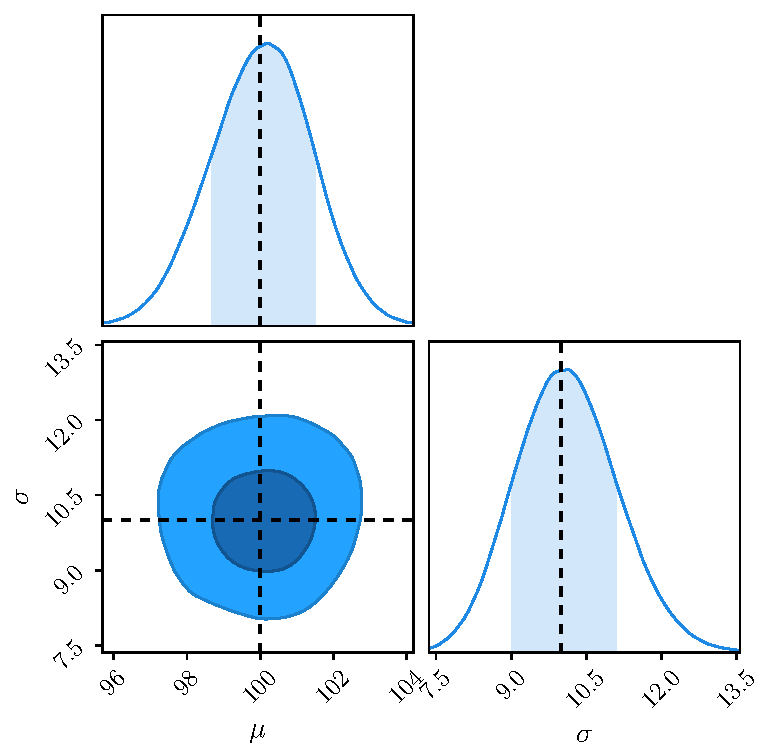
\includegraphics[width=\columnwidth]{example/perfect.pdf}
	\end{center}
	\caption{A systematic test of our perfect model, done by stacking the output chains from fitting 100 independent realisations of our 100 data points. Any systematic offset in our model would be revealed by a shift in the stacked results away from the true parameter values.}
	\label{fig:perfect}
\end{figure}


\section{The Imperfect World: Analytic Truncation}
\label{sec:imperfect}
In a slightly imperfect world we may have to deal with something like truncated data. For an example, consider the previous model, but with an instrumentation deficiency such that we can only observe events above a certain threshold, such that $x > \alpha$. I assign a value $\alpha=85$ for convenience. If we do not take this truncation into account, we will recover biased parameter estimates, as shown in Figure \ref{fig:imperfect}. However, we can correct for this truncation. If we restate our likelihood as the probability of observation given our model parameters \textit{and} our selection effects $S$, we have
\begin{align}
\mathcal{L} &= P(x | \theta, S)\\
&= \frac{P(S|x,\theta) P(x|\theta)}{P(S|\theta)}.
\end{align}
Introducing an integral over all possible data to make $P(S|\theta)$ physical,
\begin{align}
&= \frac{P(S|x,\theta) P(x|\theta)}{\int P(S, D|\theta)\, dD} \\
&= \frac{P(S|x,\theta) P(x|\theta)}{\int P(S | D, \theta) P(D|\theta)\, dD}.
\end{align}
In our example, the selection efficiency is the step function $P(S|x,\theta) = \mathcal{H}(x - \alpha)$. Having successfully observed $x$, it follows that $x > \alpha$ and so $P(S|x,\theta) = 1$. To substitute in our normal model,
\begin{align}
\mathcal{L} &= \frac{ \mathcal{N}(x|\mu, \sigma)}{\int_{-\infty}^\infty \mathcal{H}(D - \alpha) \mathcal{N}(D|\mu, \sigma)\, dD} \\
&= \frac{ \mathcal{N}(x|\mu, \sigma)}{\int_{\alpha}^\infty \mathcal{N}(D|\mu, \sigma)\, dD} \\
&= \frac{ \mathcal{N}(x|\mu, \sigma)}{\frac{1}{2} {\rm erfc}\left[ \frac{\alpha - \mu}{\sqrt{2}\sigma} \right]}, 
\end{align}
where in the last line I have evaluated the integral in the case $\mu > \alpha$. We can add this correction to our model, and note that we now recover unbiased parameter estimates, also shown in Figure \ref{fig:imperfect}.
\begin{figure}
	\begin{center}
		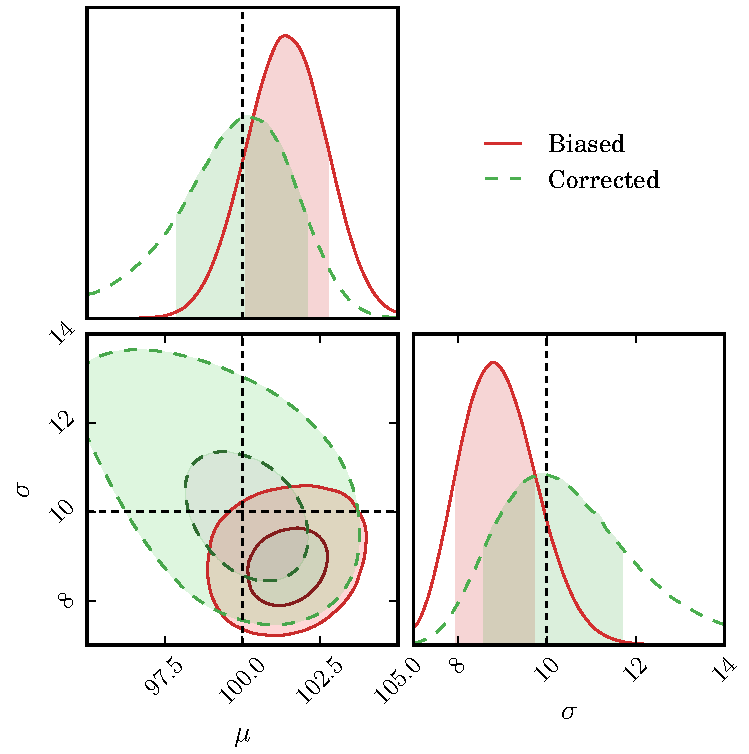
\includegraphics[width=\columnwidth]{example/imperfect.pdf}
	\end{center}
	\caption{A systematic test of our imperfect model, done by stacking the output chains from fitting 100 independent realisations of our 100 data points, subject to our thresholding. The bias shown in the red `Biased' contour can be corrected to via the techniques shown in Section \ref{sec:imperfect} to recover unbiased surfaces.}
	\label{fig:imperfect}
\end{figure}

\section{The Real World: Intractable Truncation}
\label{sec:real}
Unfortunately it is a rare scenario when dealing with nature and all her faults for us to have an analytic selection function, let alone a function encapsulated by a single parameter. A more realistic scenario involves a selection efficiency instead would take the form of non-analytic function of many model parameters. And the function would probably be stochastic too, just to throw another wrench in the works. Provided a method of forward modelling or simulating observations, the solution is to combine an analytic approximate correction with Monte Carlo integration.

So let us modify our imperfect toy model. Instead of observing just one variable, $x$, we also observe a new independent variable, $y$, which is drawn from its own distribution $y \sim \mathcal{N}(\mu_y, \sigma_y)$. Our selection efficiency can now become a combination of $x$ and $y$, such that we only observe events that satisfy $x + \beta y > \alpha$, giving $P(S|x,y,\theta) = \mathcal{H}(x + \beta y - \alpha)$.  Our likelihood for such a toy model becomes now the combination of probabilities for observing both $x$ and $y$, with the denominator becoming an integral over all possible $X$ and $Y$ observations subject to our selection effects.
\begin{align}
\mathcal{L} &= \frac{ \mathcal{N}(x|\mu, \sigma) \mathcal{N}(y|\mu_y, \sigma_y)}
{\iint_{-\infty}^\infty \mathcal{H}(x + \beta y - \alpha) \mathcal{N}(X|\mu, \sigma) \mathcal{N}(Y|\mu_y, \sigma_y)\, dX dY}
\end{align}
Assume that we cannot solve this integral analytically, and must resort to numeric solutions. These often clash with sampling methods, especially for high dimensional integrals. Inserting Monte Carlo integration into fitting algorithms can drastically slow them down, and algorithms such as Hamiltonian MCMC that require continuous surfaces can easily fail on surfaces that fluctuate from Monte Carlo integration. Even by fixing the samples used in MC integration (thereby giving a continuous surface), the complexity of the surface derivatives will pose almost insurmountable problems for any algorithms that utilise surface gradients. One solution is to find an approximate, analytic correction we can utilise in our fitting algorithm which seeks to shift the region of parameter space sampled by the sampler closer to the correct area.

In our example, if $\beta \ll 1$, such that the majority of selection effect is encapsulated by $x$ and not $y$, our approximate correction can take the form found in the previous correction from Section \ref{sec:imperfect}. Having true values of $\mu = 100$, $\sigma = 10$, $\mu_y = 30$, $\sigma_y = 5$, and a known $\beta = 0.2$, we can give a concrete example. Assuming some prior, imperfect knowledge of $\mu_y$ (perhaps we believe it is approximately $20$) we estimate that the average contribution from $\beta y$ is around $20\beta = 4$ (which is close to the correct value of $6$), and from this our analytic correction to our likelihood is
\begin{align}
w = \frac{1}{2} {\rm erfc}\left[ \frac{\alpha - \mu - 4}{\sqrt{2}\sigma} \right].
\end{align}
Further, let us explicitly break our likelihood into two parts, $\mathcal{L} = \mathcal{L}_1 \mathcal{L}_2$, with the parts given by
\begin{align}
\mathcal{L}_1 &= \frac{ \mathcal{N}(x|\mu, \sigma) \mathcal{N}(y|\mu_y, \sigma_y)}{w} \\
\mathcal{L}_2 &= \frac{ w }{\iint_{-\infty}^\infty \mathcal{H}(x + \beta y - \alpha) \mathcal{N}(X|\mu, \sigma) \mathcal{N}(Y|\mu_y, \sigma_y)\, dX dY}.
\end{align}
$\mathcal{L}_1$ can thus be fitted with a traditional sampler without numeric difficulty or slowdown, and $\mathcal{L}_2$ allows us to calculate the weight of each sample. We are effectively importance sampling our likelihood evaluations. The computational benefits of this should not be understated either - each sample in our chains can be reweighted independently, providing a task that is trivially parallelisable. Evaluating $\mathcal{L}_2$ using Monte Carlo integration of $n$ samples, we have
\begin{align}
\mathcal{L}_2 = \frac{ w n }{\sum_{i=1}^{n} \mathcal{H}(x + \beta y - \alpha) \mathcal{N}(X_i|\mu, \sigma) \mathcal{N}(Y_i|\mu_y, \sigma_y)}
\end{align}


\begin{figure}
	\begin{center}
		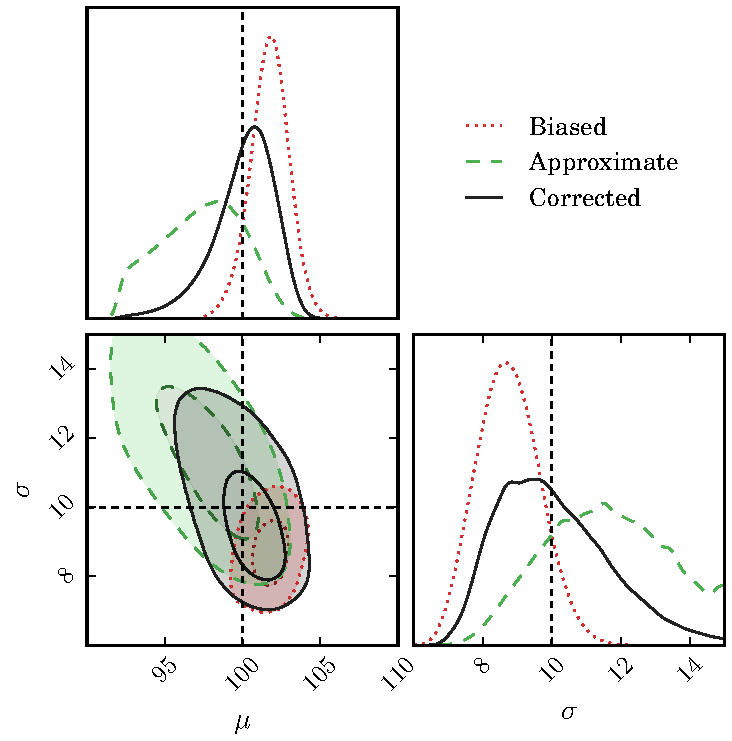
\includegraphics[width=\columnwidth]{example/real.pdf}
	\end{center}
	\caption{A systematic test of our more complicated model, done by stacking the output chains from fitting 100 independent realisations of our 100 data points, subject to our thresholding. The likelihood $\mathcal{L}_1$ was evaluated with the fitting algorithm emcee, and reweighted using Monte Carlo integration of a hundred thousand possible events as per $\mathcal{L}_2$. The truncated data with no correction is shown as `Biased' in dotted red, the `Approximate` only correction ($\mathcal{L}_1$) shown in dashed green, and the final reweighted chain shown in solid black as `Corrected'.}
	\label{fig:real}
\end{figure}
Thus we end up with a corrected posterior surface as shown in Figure \ref{fig:real}.


\section{Numerical Tricks}
\label{sec:tricks}
Further tricks can be used to increase the efficiency with which the samples are reweighted. Firstly, the overarching analytic model often provides functions which can be drawn from efficiently. In the case of our example, by drawing the random numbers $X$ and $Y$ respectively from the normal distributions $\mathcal{N}(\mu,\sigma)$ and $\mathcal{N}(\mu_y,\sigma_y)$ (ie traditional importance sampling) we need only evaluate the step function for our data points.


If evaluating the probability that an event is observed is numerically expensive (i.e. not a step function), it is easy to pregenerate a set of events and reuse them for all weights - provided that the number of events used when calculating the weights is sufficient to make the statistical error of Monte Carlo integration insignificant when compared to the constraining power of your dataset. This method is however only efficient when prior knowledge of parameter values is known to allow a reasonable initial draw of events. Without this prior information, samples need to span the entire posterior volume, which is numerically intractable even for low dimensional models.





\section{Conclusion}
\label{sec:conclusion}



Reword the abstract or similar


\section*{Acknowledgments}

We gratefully acknowledge the input of the many researchers that were consulted during the creation of this paper.


\bibliography{bibliography}


% Don't change these lines
\bsp	% typesetting comment
\label{lastpage}
\end{document}

% End of mnras_template.tex

